%\documentclass[manuscript]{aastex}
\documentclass[]{emulateapj}
%-- Packages 
\usepackage[backref, breaklinks, colorlinks, citecolor=blue, linkcolor=magenta]{hyperref}
\usepackage[dvipsnames]{xcolor}


\newcommand{\vdag}{(v)^\dagger}
\newcommand{\myemail}{sanchenn@uw.edu}

\slugcomment{Submitted to The Astrophysical Journal}

\shorttitle{BH Driven \ion{O}{6} in the CGM}
\shortauthors{Sanchez et. al.}

\usepackage{natbib}
%\bibliographystyle{plain}
\bibliographystyle{apj}

\begin{document} 

%\title{Some like it HOT: Touring the CGM of Simulated Milky Way Type Galaxies}
%\title{Metals on the BH Express: AGN Feedback Transported \ion{O}{6} in the Simulated CGM of Milky Way-Mass Galaxies}
%\title{Metals on the BH Express: Oxygen Transport in the CGM of Simulated MW-Mass Galaxies}
\title{Not So Heavy Metals:  Black Hole Feedback Enriches The Circumgalactic Medium}
%\title{Not So Heavy Metals: Oxygen Transport via Black Hole Feedback in the Circumgalactic Medium}



\author{N. Nicole Sanchez\altaffilmark{1}}
\author{Jess Werk\altaffilmark{1}}
\author{Michael Tremmel\altaffilmark{2}}
\author{Andrew Pontzen\altaffilmark{3}}
\author{Charlotte Christensen\altaffilmark{4}}
\author{Tom Quinn\altaffilmark{1}}
\author{Akaxia Cruz\altaffilmark{1}}
\author{[\textbf{Order subject to change}]}
%\author{Marta Volonteri\altaffilmark{7}}
%\author{James Wadsley\altaffilmark{8}}


\affil{$^1$Astronomy Department, University of Washington, Seattle, WA 98195, US, sanchenn@uw.edu}
\affil{$^2$Yale Center for Astronomy \& Astrophysics, Physics Department, P.O. Box 208120, New Haven, CT 06520, USA}
\affil{$^3$Department of Physics \& Astronomy, University College London, 132 Hampstead Road, London, NWI 2PS, United Kingdom}
\affil{$^4$Physics Department, Grinnell College, 1116 Eighth Ave., Grinnell, IA 50112, United States}

%\affil{$^2$ Yale I guess}
%\affil{$^3$ Somewhere in England}
%\affil{$^6$Department of Physics and Astronomy, Rutgers, The State University of New Jersey, 136 Frelinghuysen Road,Piscataway, NJ 08854, USA}
%\affil{$^7$Institut d’Astrophysique de Paris, Sorbonne Universitès, UPMC Univ Paris 6 et CNRS, UMR 7095, 98 bis bd Arago, 75014 Paris, France}
%\affil{$^8$Department of Physics and Astronomy, McMaster University, Hamilton, ON L8S 4M1, Canada}


% #####################################
% ############# ABSTRACT ##############
% #####################################

\begin{abstract}\label{abs:abstractlabel}

%The CGM is where most of the gas mass of galaxies lay [CITE]. It is important to examine the evolution of the CGM and see how changes in the galaxy may effect this large reservoir of gas as it has direct consequences on the continued evolution of the galaxy. We examine a suite of genetically modified Milky Way-mass galaxies to pin point the effects on the CGM that small and large scale changes to a galaxy may cause. By determining what modifications to a Milky Way-type simulated galaxy results in the most MW like galaxy and furthermore examining what characterizes the CGM of that galaxy, we take a step closer to better understanding the elusive CGM of our own galaxy. 
 
By tracing the redistribution of metals in the circumgalactic medium (CGM) via outflows, we show that \ion{O}{6} is a sensitive indicator of supermassive black hole (SMBH) feedback. We examine the effects of SMBH feedback on the CGM using a cosmological hydrodynamic simulation \citep[{\sc Romulus25} ][]{Tremmel2017} and a set of zoom-in ``genetically modified'' Milky Way-mass galaxies sampling different evolutionary paths. We compare the column densities of \ion{O}{6} in Milky Way-mass galaxies and compare them with observations from the COS-Halos Survey; contrary to previous simulations which underpredicted the CGM column densities of \ion{O}{6}, these simulations are consistent with COS-Halos observations of star forming galaxies and slightly overpredict \ion{O}{6} in quenched galaxies. We determine that a galaxy's star formation history and overall accretion rate have little effect on the appearance of \ion{O}{6} in its CGM while column densities of \ion{O}{6} are more closely tied to galaxy halo mass and BH growth history. The set of zoom-in, genetically modified Milky Way-mass galaxies confirm that the SMBH acts as the physical mechanism for transporting metals out into its host halo thereby significantly impacting the column densities of \ion{O}{6} found in the CGM. 

\end{abstract}
\keywords{Gas physics -- Galaxies: circumgalactic medium -- Galaxies: spiral -- Galaxies: kinematics and dynamics -- Methods: Numerical}


% ########## END OF ABSTRACT ##########
% #####################################


% #####################################
% ########## INTRODUCTION #############
% #####################################

\section{Introduction} 
\label{sec-intro}

% The  link between metals and which phase they’re excited to in  the CGM is uncertain. The CGM is clearly part of the recycling/growth of a galaxy.
%	Oppenheimer, Suresh, COS-halo, Werk, Tumlinson, Peeples (probably?)
The circumgalactic medium (CGM), the extended region of gas surrounding galaxies out to their virial radii, is richly structured with the by-products of galaxy evolution. Due to its diffuse nature, the CGM remains one of the most difficult regions to observe. Beginning in 2010, targeted observations of the CGM began in earnest due to technological advances like the Cosmic Origins Spectrograph (COS) on the Hubble Space Telescope (HST). Most observations have focused on UV and optical lines, using a variety of methods. COS-Halos is one such survey which uses the light of distant quasars to probe the absorption lines of CGM gas within galaxies in a quasar's line of sight. Other methods include: stacking analyses, which combine hundreds or thousands of spectra to parse out the faint signals of CGM lines \citep{York2006,Peek2015,Steidel2010}; ``down-the-barrel'' spectroscopy, which employs a galaxy's own starlight as the background source for CGM absorption \citep{Martin2006,Bordoloi2011,Rubin2014,Heckman2015}; and emission line maps, which search for the few photons emitted directly by CGM gas \citep{Putman2012a,Hayes2016}. Emission line maps and absorption line studies have also been made in X-ray, and additional X-ray observations by Chandra and XXM have been used to help constrain the extent of the CGM \citep{Nicastro2005}. Through these studies, observers have found the CGM region to be a structurally complex, multiphase medium \citep{Tumlinson2011,Werk2012,Werk2013a,Werk2016,Tumlinson2017}. \cite{Werk2014} show that most of the ``missing baryons'' of galaxies likely reside in this diffuse region, implying that the CGM may play a key role in the growth of galaxies and the build up of their disks. Therefore, it is clear that understanding the CGM is crucial for understanding the complex nature of galaxy evolution and growth. 

% GXY evolution is thought to imprint itself on the CGM
Widespread \ion{O}{6} absorption in halos has presented a particularly intriguing puzzle for theorists. COS-Halos finds a correlation between the column densities of \ion{O}{6} out to 150 kpc and the specific star formation rate (sSFR) of their observed galaxies. Higher column densities of \ion{O}{6} are found around SF galaxies compared to their passive counterparts. \cite{Oppenheimer2016} argue that this bimodality arises due to the \ion{O}{6} acting as a proxy for the virial temperature of gas in these galaxy halos. Therefore, more massive galaxies have more of their oxygen in a phase traced by \ion{O}{7} and \ion{O}{8}; thus, the COS-Halos sample show less \ion{O}{6} in their CGM due to the intrinsically higher virial temperature of these massive red ellipticals. In contrast, \cite{Suresh2017} argue that the \ion{O}{6} is built up by SMBH feedback, which can physically modify the CGM via outflows or heat it to the appropriate temperature for ionizing \ion{O}{6}. In both cases, each argument implies an intrinsic link between the CGM and its host galaxy's evolution. 

% As the growth mechanisms of the AGN and galaxy are intrinsically linked, we also consider the evolution of these galaxies and the role of evolution on the Cgm structure. The AGN is thought to have a direct effect on CGM of host galaxies.
Additionally, galaxy evolution has been shown to be strongly tied to the evolution of its central supermassive black hole (SMBH). Through relations like the M-$\sigma$ and the bulge mass-BH mass correlation \citep{Ferrarese2000,Mcconnell2013}, recent studies indicate that the SMBH and its host galaxy halo \textit{co-evolve} \citep[][and references therein]{Gebhardt2000,Volonteri2012b,Kormendy2013,Reines2015c}.   It is therefore unsurprising that a SMBH is thought to leave its marks on the CGM. However, the direct mechanisms by which the SMBH impacts the CGM are still debated. 

% Could it be the AGN heating the CGM or the AGN physically driving out gas or the AGN not driving out metals?
SMBHs may effect the CGM in a variety of ways. First, feedback from the active SMBH may inject energy into the surrounding material, raising temperatures, and ionizing metals in the gas \citep{McQuinn2017,Mathews2017,Oppenheimer2018}. Additionally, massive outflows of gas from the SMBH may physically push gas out of the galaxy. Some of this gas may end up falling back into the galaxy as part of the ``recycling'' of the CGM \citep{Tumlinson2017}, enriching CGM gas with metals from the center of the galaxy, and further enriching the IGM as gas is expelled from the galaxy halo.  

% Simulations have evolved to help us understand the underlying physics of observations.
Cosmological hydrodynamic simulations have become a powerful tool for examining the physics driving the multiphase nature of the CGM \citep{Cen2013,Ford2016b,Oppenheimer2016,Suresh2017,Nelson2018}. Simulators have long been examining the underlying physics of SMBH activity in galaxies; however, recent studies have proven that the observed properties of the CGM are not easily matched and the underlying physics of this region is a fairly new field, ripe for discovery. Most previous studies have underpredicted the column densities of \ion{O}{6} found by COS-Halos  \citep[including the aforementioned studies,][]{Oppenheimer2008,Suresh2017}; however, important strides have started to be made in probing this diffuse region. Using the smooth particle hydrodynamic code GADGET-2 \citep{Springel2005a,Oppenheimer2008}, \cite{Ford2016a} found that the presence of \ion{O}{6} in the CGM likely arises from metals ejected early on in the galaxy's evolution. More recently, \cite{Nelson2018} well-matched the COS-Halos observations using the IllustrisTNG simulations and determined that the amount of \ion{O}{6} the the CGM can depend on a variety of galactic properties including sSFR. In particular, they determine that BH feedback (specifically, their low-accretion, kinetic-feedback mode) plays a crucial role in setting the amount of \ion{O}{6} in the CGM by affecting the amount of metal mass ejected by their galaxy.

We continue this ongoing investigation of the CGM using two sets of simulations: the cosmological volume, {\sc Romulus25} \citep{Tremmel2017} and three ``genetically modified'' variations of an isolated, zoom-in Milky-Way (MW) mass galaxy \citep{Roth2016,Pontzen2016} simulated with and without the implementation of BH physics. Additionally, we compare properties of these simulations with the COS-Halos Survey. Though other observational surveys have examined the CGM around galaxies \citep{Stocke2013,Borthakur2015,Danforth2016}, COS-Halos \citep{Tumlinson2011} remains the best-studied, uniformly-selected sample of isolated, MW-mass host galaxies to-date. Their readily available gas column densities and the galaxy properties in the survey allows us to directly compare with these observations. 

With our set of simulations and these observational comparisons, we examine the effects of both environmental and internal galaxy processes on the physical state and content of the CGM. Specifically, we address:\\
\\
$\bullet$ How the star formation and accretion history of the galaxy co-evolve with the CGM \\
$\bullet$ How SMBH activity imprints itself on the CGM \\
\\
%First, we examine the CGM in a range of MW-mass galaxies with varied morphologies from {\sc Romulus25} . Additionally, from a cosmological volume, we selected a Milky Way-analog based on halo mass for our zoom-in simulations. From this isolated MW-mass galaxy and its subsequent ``genetic modifications'', we quantify the effect of SMBH feedback on the CGM by examining a set of star forming and passive galaxies run both with and without BH physics. 
Using these isolated, zoom-in simulations in tandem with the {\sc Romulus25}  simulation, we illuminate the roles that stellar evolution and SMBH feedback play in setting the properties of the CGM of MW-mass galaxies.

In Section \ref{sec-model}, we describe the underlying physics used in our two galaxy samples. Section \ref{sec-results} details our results from examining the CGM in ROMULUS25 and comparisons with the zoom-in galaxies. We discuss these results and their implications for future studies in Section \ref{sec-discuss}. In Section \ref{sec-conclude}, we summarize and offer conclusions. 

%The latter of these we have genetically modified to result in a suite of four isolated galaxies, two of which are star forming and two of which are quenched.  \\

% We want to examine two questions with our simulations

% First, how does the evolution of the galaxy imprint itself on the CGM (if it does at all)

% Second, how the the BH imprint itself on the CGM

% We use Romulus25 a cosmological volume with [SPECS] to examine the CGM in a range of galaxy morphologies all within the MW mass regime. (Define “MW mass regime”)
%	Halo mass histogram (highlight MW mass range)

% To further examine the morphological effect on the CGM, we examine a Patient 0 simulation with 3 genetic modifications, which results in four simulations of the same galaxy with minor changes, two of which are star forming and 2 of which are quenched. All are within the MW mass range described above.
%	Diagram with density image of galaxies, halo mass, R_vir, satellite mass, NEW NAME


%In addition to the work of Oppenheimer and Suresh, Ford et al 2016 shows that the implementation of different types of galactic wind feedback results in passive galaxies without distinctly altering the CGM. (Ref later?) \textbf{[MORE EXAMPLES]} 

% Introduce Romulus and GM, here’s what we’re going to answer this questions about how oxygen makes it to the CGM in the \ion{O}{6} state.


%\textbf{Outline in Bold:} \\
%\textbf{Intro 1: Discuss CGM} \\

%Since 2011, the circumgalactic medium (CGM) has emerged as one of the final, unexplored frontiers for understanding galaxy evolution in the low-z universe. Understanding its phase structure, dynamics, and overall relationship to its host galaxy is now of critical importance to making progress. The CGM is a gaseous halo surrounding a galaxy through which incoming gas passes as it flows from the intergalactic medium onto galaxy disks. While the CGM hosts some of the most observationally elusive particles in the universe, studies of this medium suggest that it is multi-phase, highly dynamic, and dominated by complex ionization processes [CITE]. The CGM also maintains a reservoir of gas that is simultaneously being accreted onto the galactic disk and outflowing from the galaxy through stellar and supermassive black hole (SMBH) feedback [CITE, Michael, Fabio, Jillian]. This recycling of gas into and out of the galaxy serves to both fuel the galaxy’s star formation and to quench its activity. It is clear that the CGM plays a pivotal role in the formation and evolution of its host galaxy [CITE]; however, there are many questions about the CGM that continue to elude astronomers. Such as, how does baryonic content and ionization state depend on the activity of the galaxy host, particularly SMBH feedback? And also, how does baryonic content and ionization state depend on galaxy assembly history?

%\begin{figure}
%\centerline{\resizebox{0.95\hsize}{!}{\includegraphics[angle=0]{Jess_plot}}}
%\caption[]{.}
%\label{}
%\end{figure}

%Related to the mysteries posed by the CGM, astronomers are also trying to understand how the quenching of galaxies, that is the ``turning off'' of star formation that leads to red elliptical galaxies, occurs. In particular, what causes galaxies to quench, and what sustains their lack of star formation? Some considerations of this dilemma include staunching IGM accretion which feeds the CG[cite, observations and sims!] and effects which keep the CGM hot enough that stars are unable to form, such stellar or AGN feedback or \textit{major?} mergers with other galaxies [Pontzen2017, cite more]. 

%Observationally, one common method of investigating the CGM is through line of sight observations of background QSOs. Studying the spectra of bright background objects allows us to examine the absorption features of the extended foreground gaseous media (including the CGM
%of galaxies nearby in projection) through which the QSO’s light filters [FIGURE?]. These absorption-line studies allow for the direct measurement of absorption features (characterizing the CGM) within the QSO spectra, allowing us to study the elusive CGM more directly. 

%\textbf{Intro 2: Discuss NBODY Sims} \\

%Cosmological hydrodynamic simulations are an important tool for understanding the underlying physics characterizing the CGM. Current smooth particle hydrodynamic (SPH) simulations utilize a dark-matter-only component and a follow-up zoom-in simulation to bridge the gap between large-scale galactic gravitational effect and the small-scale effects of gas, stars, and dust. Significant discoveries have already been made by investigating the CGM of simulated galaxies. Ford et al. (2013) determined that 65 -- 80 percent of the total baryon mass of a galaxy exists in the halo outside the stellar disk and that $\sim$80$\%$ of the fuel for star formation in the Milky Way Galaxy was in the CGM 1 billion years ago. However, most comparisons between simulation and data have primarily focused on bulk column density comparisons and largely ignored gas kinematics \citep {Stinson2012, Hummels2013, Ford2016a, Oppenheimer2016, Suresh2017}

%One of the most high resolution and recent cosmological simulation codes, ChaNGA, is a smoothed-particle hydrodynamics (SPH) code, which can directly examine the dynamics of the CGM in its simulated galaxies. Though comparable to the “Eris” simulations in mass and force resolution, ChaNGa has higher reliability when resolving high-density regions (Zolotov2012) and an improved implementation of black hole (BH) accretion, dynamics, and formation (Tremmel2016). These simulations allow us to determine kinematic information about the gas and metals residing in the CGM of these simulated galaxies and how it is affected by the BH and AGN activity. 

%\textbf{Intro 2: Discuss GM Sims} \\

%These “genetically modified” (GM) simulations of low redshift galaxies keep the large scale structure and cosmological conditions of $\alpha$ CDM consistent, while allowing for modifications of their accretion histories (Roth2015, more?). The analyses of these GM simulations allow for direct comparisons of the CGM of multiple versions of the same galaxy in a physically self-consistent treatment. Previous studies have  inspected the quenching mechanisms that arise from these varied accretion histories \citep{Pontzen2017}; however, they have not yet examined the dynamical effects on the CGM gas that these modified accretion histories generate.

%These genetically modified galaxies serve to further examine the questions posed by the CGM and its relation to quenching. We can look to the changes or similarities in the CGM amidst this suite of simulations to see how the subtle changes made to each of these Milky Way galaxies affect the CGM in a self-consistent way.

%The simulation parameters of the individual GM galaxies are described in Section 2. Simulation analysis methods are described in Section 3. Results are compiled in Section 4, and we summarize our findings in Section 5.


% ####### END OF INTRODUCTION #########
% #####################################


% #####################################
% ####### SIMULATION PARAMETERS #######
% #####################################

\section{Simulation Parameters}\label{sec-model}

% BELOW IS DM MASS TABLE; PROBABLY UNNECCESSARY
% \begin{table}[ht] % `*' makes it go across both columns instead of one
% \caption{Gas+BH Simulation Details} % title of Table
% \centering % used for centering table
% \begin{tabular}{c c c} % centered columns (4 columns)
% \hline\hline %inserts double horizontal lines
% Sim & Total Halo Mass & R$_{vir}$\\
%  & (M$_{\odot}$) & (kpc) \\ [0.5ex] % inserts table
% %heading
% \hline % inserts single horizontal line
% P0 & 9.91 $\times$ 10$^{11}$ & 262.3\\ % inserting body of the table
% GM1 & 1.02 $\times$ 10$^{12}$ & 264.5\\
% GM4 & 8.58 $\times$ 10$^{11}$ & 250.0\\
% GM5 & 9.08 $\times$ 10$^{11}$ & 254.7\\
% GM6 & 7.58 $\times$ 10$^{11}$ & 239.8\\ [1ex] % [1ex] adds vertical space
% \hline %inserts single line
% \end{tabular}
% \label{table:nonlin} % is used to refer this table in the text
% \end{table}

%Romulus & GMs: NO METAL LINE COOLING
%   Galaxy masses: mass-metallicity, M-sigma, SMHM
%	Cooling mechanisms
%	BH seeding and formation requirements, mergers: Michael!
%	Accretion model: Tremmel 2016
%	BH feedback
%	Dynamical friction: Tremmel 2015

\subsection{ChaNGa Physics} 
Both {\sc Romulus25}  (hereafter R25) and our set of zoom-in galaxies were run using the smoothed particle hydrodynamics N-body tree code, Charm N-body GrAvity solver \citep[ChaNGa,][]{Menon2015}. ChaNGa includes the same models for a cosmic UV background, star formation (using a Kroup IMF), `blastwave' SN feedback, and low temperature metal line cooling as previously used in GASOLINE \citep{Wadsley2004,Wadsley2008,Stinson2006,Shen2010}. Neither {\sc Romulus25}  or the zoom-in simulations utilize H2 cooling as the resolution of these simulations is to large to consider individual star forming regions. ChaNGa includes an improved SPH formalism which includes a geometric density approach in the force expression. This update to the hydrodynamic treatment includes thermal diffusion \citep{Shen2010} and reduces artificial surface tension allowing for better resolution of fluid instabilities \citep{Ritchie2001,Menon2015,Governato2015}. 

Additional improvements have been made to the BH formation, accretion, and feedback models as well an improved prescription for dynamical friction \citep{Tremmel2015,Tremmel2017}. BH seed formation is tied to dense, extremely low metallicity gas to better estimate SMBH populations in a wide range of galaxies. Sub-grid models for both dynamical friction \textemdash to better simulate realistic SMBH dynamical evolution and mergers \textemdash and accretion have been implemented. The new SMBH accretion model considers angular momentum supported gas from nearby gas allowing for more physical growth compared to Bondi-Hoyle prescription alone or other methods that require additional assumptions or free parameters \citep{Rosas-Guevara2015,Angles-Alcazar2017}. Angular momentum support is taken into account in the accretion equation:
\begin{equation}
\dot{M} \sim \frac{\pi (GM)^2 \rho c_s}{(v_{\theta}^2 + c_s^2)^2},
\end{equation}
where $v_{\theta}$ is the rotational velocity of the gas surrounding the BH and is informed by the angular momentum support of the gas on the smallest, resolvable scale. However, when bulk motion dominates over rotational motion, the formula reverts to the original Bondi-Hoyle.
SMBH feedback energy is imparted on the nearest 32 particles gas particles according to a kernel probability and is determined by the accreted mass, $\dot{M}$, as: 
\begin{equation}
E = \epsilon_{r} \epsilon_{f} \dot{M} c^2 dt, 
\end{equation}
where $\epsilon_{r}$ = 0.1 and $\epsilon_{f}$ = 0.02 are the radiative and feedback efficiency, respectively, and $dt$ represents one black hole timestep, during which the accretion is assumed to be constant.  

All our simulations were run with a $\Lambda$CDM cosmology from the most recent Planck collaboration utilizing $\Omega_m$ = 0.3086, $\Omega _{\Lambda}$ = 0.6914, h = 0.67, $\sigma_8$ = 0.77 and have Plummer equivalent force softening lengths of 250 pc. For simulating the cosmic reionization energy, both simulations have a UV background at z $\sim$ 9 \citep{Haardt2012}.

\subsection{{\sc Romulus25}  Cosmological Volume}
The {\sc Romulus25}  \citep[][R25]{Tremmel2017} simulation is a cosmological volume which includes galaxy halos within the mass range 10$^{9}$ \textemdash 10$^{13}$ M$_{\odot}$. R25 has a mass resolution of 3.4 $\times$ 10$^5$ M$_{\odot}$ and 2.1 $\times$ $10^5$ M$_{\odot}$ for DM and gas particles, respectively. Galaxies in R25 have been shown to lie along the M-$\sigma$ and SMHM relation (Figure \ref{fig-massmetal}), and are consistent with observations of star formation and SMBH accretion histories at high redshift \citep{Tremmel2015}. Additionally, \cite{Tremmel2015} shows that SMBH physics is a necessary component for reproducing the evolution of MW-mass galaxies as well as quenching in massive galaxies. For our study, we focus on the galaxies in R25 that fall within the stellar mass range of COS-Halos: 3 $\times$ 10$^{10}$ M$_{\odot}$ and 3 $\times$ $10^{11}$ M$_{\odot}$. We examine all the galaxies within the specified mass range. % and exclude any galaxies within twice the virial radius of another galaxy, thereby removing galaxies that might be satellites of a larger galaxy. 
With these selection criteria in place, our sample includes 52 (without excluding possible satellite galaxies). Using the sSFR cut of COS-Halos, 46 of these galaxies are star forming (sSFR \textless \ 1.6 $\times$  10$^{-11}$ M$_{\odot}$  yr$^{-1}$) and 6 are passive at z $\sim$ 0.17. We note that this is a conservative estimate using the corrections from {Munshi 2013}. However, by z = 0, the quenched fraction is about 50 \%. We use the factor of 1.6 to account for the fact that COS-Halos uses a Sal-Peter IMF while our simulations use a Kroupa IMF \citep{Kroupa1993}.

\begin{figure}[]
\centerline{\resizebox{1.02\hsize}{!}{\includegraphics[angle=0]{ROM_Mstellar_Mhalo}}}
\caption[]{R25 is an SPH simulated cosmological volume with galaxy halos spanning the orders of 10$^{9}$ \textemdash 10$^{13}$ M$_{\odot}$. We show that the 52 galaxies in our sample, which are selected within the stellar mass range of COS-Halos, fall well within the stellar mass-halo mass (SHMH) relation. Red squares and blue circles represent passive and star forming galaxies, respectively.}
\label{fig-massmetal}
\end{figure}


\begin{figure}[]
\vspace{-2mm}
\centerline{\resizebox{1.02\hsize}{!}{\includegraphics[angle=0]{P0_faceon_gas}}}
\vspace{0mm}
\centerline{\resizebox{1.02\hsize}{!}{\includegraphics[angle=0]{P0_edgeon_gas}}}
\caption[]{A face-on and edge on gas density image of our initial Milky Way-mass galaxy, Patient 0, at z = 0.}
\label{fig-P0}
\end{figure}

\subsection{Zoom-In Galaxies: Patient 0 and its Genetic Modifications}
While R25 gives cosmological context to our analysis, we examine our set of genetically modified zoom-in galaxies to better understand the physical mechanisms at play. To select our galaxy, we ran initial uniform-volume, 50 h$^{-1}$ Mpc on a side, dark matter-only cosmological volume. From this volume, we selected an isolated MW-mass (M$_{vir}$ = 9.9 $\times$ 10$^{11}$) halo at z=0 as our ``Patient 0'' (hereafter P0) and then re-simulated it at a higher resolution with baryons. We additionally required that the galaxy be \textgreater 2 Mpc away from another MW- or higher mass galaxy and selected it for the satellite galaxy contained within its virial radius at z = 0. Selecting a MW-mass galaxy allows us to compare directly with the COS-Halos observations, which observed $\sim$ L$^{*}$ galaxies. For the subsequent, ``genetically modified'' (GM) zoom-in runs, we use the method of genetic modification of \cite{Pontzen2016} which creates a set of very similar initial conditions that result in subsequent galaxy simulations which keep the large scale structure and cosmological conditions $\Lambda$CDM consistent (as in P0), while resulting in slight modifications to their accretion histories \citep{Roth2016}. For our purposes, we decreased the mass of the satellite which exists at z = 0 in P0 and shrank its mass \textit{prior} to when it enters the galaxy at z = 1. To create the modified set of initial conditions, we determined which elements in the linear overdensity field of the initial condition grid map to the particles in the satellite. We then decreased the mean overdensity of these elements in the initial linear vector, all the while, maintaining the mean overdensity of the elements mapping to the main halo to preserve the final mass. 

Patient 0 (and its 3 GM simulations) have a mass resolutions of 1.4 $\times$ 10$^5$ M$_{\odot}$ and 2.1 $\times$ $10^5$ M$_{\odot}$ for DM and gas particles, respectively. The DM field in these galaxies is simulated at twice the gas linear resolution to reduce noise in the potential near the galactic center \citep{Pontzen2016} and more accurately trace black hole dynamics \citep{Tremmel2015}.

\subsubsection{Galaxies with BH Physics} 

\vspace{-5 mm}
\begin{table}[ht] 
\caption{Zoom-In Galaxies Modifications \textbf{at z = 1}} % title of Table
\centering % used for centering table
\begin{tabular}{c c} % centered columns (4 columns)
\hline\hline %inserts double horizontal lines
Sim & Satellite Dark Matter Mass \\
 & (M$_{\odot}$)\\ [0.5ex] % inserts table
%heading
\hline % inserts single horizontal line
P0 $\&$ noBH & 7.3 $\times$ 10$^{10}$ \\ % inserting body of the table
GM1 $\&$ noBH & 5.9 $\times$ 10$^{10}$ \\
GM2 $\&$ noBH & 4.0 $\times$ 10$^{10}$ \\ % This used to be GM7
GM3 $\&$ noBH & 2.5 $\times$ 10$^{10}$ \\ [1ex] % [1ex] adds vertical space; GM3 used to be GM4
\hline %inserts single line
\vspace{0mm}
\end{tabular}
\label{table:satdata} % is used to refer this table in the text
\end{table}

\begin{table*}[ht!] % `*' makes it go across both columns instead of one
\caption{Zoom-In Galaxies Properties \textit{with BHs} at \textbf{z = 0.17}} % title of Table
\centering % used for centering table
\begin{tabular}{c c c c c c c} % centered columns (4 columns)
\hline\hline %inserts double horizontal lines
Sim & Total Halo Mass  & Total Gas Mass & Total Stellar Mass & CGM Gas Mass & R$_{vir}$ & T$_{vir}$ \\
 & (M$_{\odot}$) & (M$_{\odot}$) & (M$_{\odot}$) & (M$_{\odot}$) & (kpc) & (K) \\ [0.5ex] % inserts table
%heading
\hline % inserts single horizontal line 
P0 & 9.9 $\times$ 10$^{11}$ & 1.1 $\times$ 10$^{11}$ & 5.0 $\times$ 10$^{10}$ & 9.3 $\times$ 10$^{10}$ & 277.0 & 5.5 $\times$ 10$^5$ \\ 
GM1 & 9.7 $\times$ 10$^{11}$ & 9.9 $\times$ 10$^{10}$ & 4.7 $\times$ 10$^{10}$ & 8.5 $\times$ 10$^{10}$ & 274.9 & 5.4 $\times$ 10$^5$ \\
GM2 & 8.1 $\times$ 10$^{11}$ & 6.9 $\times$ 10$^{10}$ & 1.4 $\times$ 10$^{10}$ & 6.9 $\times$ 10$^{10}$ & 259.2 & 4.8 $\times$ 10$^5$ \\ % This used to be GM7
GM3 & 6.6 $\times$ 10$^{11}$ & 5.1 $\times$ 10$^{10}$ & 1.1 $\times$ 10$^{10}$ & 5.1 $\times$ 10$^{10}$ & 241.7 & 4.2 $\times$ 10$^5$ \\ [1ex] % [1ex] adds vertical space; GM3 used to be GM4
\hline %inserts single line
\end{tabular}
\label{table:BHdata} % is used to refer this table in the text
\vspace{-2mm}
\end{table*}

\begin{table*}[ht] % `*' makes it go across both columns instead of one
\caption{Zoom-In Galaxies Properties \textit{without BHs} at  \textbf{z = 0.17}} % title of Table
\centering % used for centering table
\begin{tabular}{c c c c c c c} % centered columns (4 columns)
\hline\hline %inserts double horizontal lines
Sim & Total Halo Mass  & Total Gas Mass & Total Stellar Mass & CGM Gas Mass & R$_{vir}$ & T$_{vir}$\\
 & (M$_{\odot}$) & (M$_{\odot}$) & (M$_{\odot}$) & (M$_{\odot}$) & (kpc) & (K) \\ [0.5ex] % inserts table
%heading
\hline % inserts single horizontal line
P0noBH & 9.8 $\times$ 10$^{11}$ & 8.2 $\times$ 10$^{10}$ & 7.9 $\times$ 10$^{10}$ & 7.5 $\times$ 10$^{10}$ & 276.1 & 5.4 $\times$ 10$^5$ \\ % inserting body of the table
GM1noBH & 9.9 $\times$ 10$^{11}$ & 8.7 $\times$ 10$^{10}$ & 7.4 $\times$ 10$^{10}$ & 8.0 $\times$ 10$^{10}$ & 276.2 & 5.5 $\times$ 10$^5$ \\
GM2noBH & 9.6 $\times$ 10$^{11}$ & 8.8 $\times$ 10$^{10}$ & 7.0 $\times$ 10$^{10}$ & 8.0 $\times$ 10$^{10}$ & 274.0 & 5.3 $\times$ 10$^5$ \\ % This used to be GM7
GM3noBH & 8.4 $\times$ 10$^{11}$ & 7.1 $\times$ 10$^{10}$ & 7.3 $\times$ 10$^{10}$ & 6.4 $\times$ 10$^{10}$ & 261.9 & 4.9 $\times$ 10$^5$ \\ [1ex] % [1ex] adds vertical space; GM3 used to be GM4
\hline %inserts single line
\vspace{5.111mm}
\end{tabular}
\label{table:noBHdata} % is used to refer this table in the text
\end{table*}


At z = 0, our P0 galaxy is a star forming galaxy with a disk (Figure \ref{fig-P0}). P0 has an incoming satellite at z = 0 with an original mass of 7.34 $\times$ 10$^{10}$ M$_{\odot}$ (mass ratio, q = 0.12) \textit{prior} to entering the main halo's virial radius at z $\sim$ 1. For each GM galaxy simulation, we systematically shrink this satellite halo's mass prior to its entry with the main halo (Table \ref{table:satdata}). GM1 results in a similar disked, star forming galaxy as P0, while GM2 and GM3 become quenched at z $\sim$ 1 (Table \ref{table:BHdata}).

%\textit{GM1:} For our first GM galaxy, we shrink the satellite halo's mass to 5.86 $\times$ 10$^{10}$ M$_{\odot}$ (q = 0.10). At z = 0, GM1 is a star forming galaxy (Figure \ref{sfh}a) with a disk and has a final halo mass of 1.07 $\times$ 10$^{12}$ and R$_{vir}$ = 269 kpc. It has total gas and stellar masses of 1.01 $\times$ 10$^{11}$ M$_{\odot}$ and 6.43 $\times$ 10$^{10}$ M$_{\odot}$, respectively.

%\textit{GM2:} Our second GM galaxy has a incoming satellite mass shrunk to 3.97 $\times$ 10$^{10}$ M$_{\odot}$ (q = 0.06). At z = 0, GM2 has a final halo mass of 8.69 $\times$ 10$^{11}$ M$_{\odot}$ and R$_{vir}$ = 254 kpc. It has total gas and stellar masses of 7.41 $\times$ 10$^{10}$ M$_{\odot}$ and 1.38 $\times$ 10$^{10}$ M$_{\odot}$, respectively.

%\textit{GM3:} The third and final GM galaxy has a incoming satellite mass shrunk to 2.45 $\times$ 10$^{10}$ M$_{\odot}$ (q = 0.04). At z = 0, GM3 has a final halo mass of 7.76 $\times$ 10$^{11}$ M$_{\odot}$ and R$_{vir}$ = 242 kpc. It has a total gas and stellar masses of 6.36 $\times$ 10$^{10}$ M$_{\odot}$ and 1.04 $\times$ 10$^{10}$ M$_{\odot}$, respectively. 

While these GM galaxies are generated using the same method as \cite{Pontzen2016}, their study examines a different set of galaxies. The three galaxies in \cite{Pontzen2016} were run to z = 2 and have M$_{Halo}$ $\sim$ 10$^{12}$. They each have incoming satellites whose masses are both increased and decreased prior to merging with the main galaxy, as in our galaxies; however, the resulting effect of their modifications were different from ours, as we explore in Section \ref{subsec-quench}.

\subsubsection{Galaxies without BH Physics}
One key benefit of the individual zoom-in galaxies includes the ability to remove or adjust the physical parameters affecting our galaxies. This capability allows us to test different theoretical models which would be too computationally expensive to do with a large volume like R25. In particular, we may exploit this utility to understand directly the effects of the SMBH. To isolate the effect of the SMBH on the CGM, all four of the zoom-in simulations (P0 and its 3 GMs) were re-simulated at the same resolution and with all the same physics \textit{excluding} BH formation, feedback, and dynamical friction (Table \ref{table:noBHdata}). Black hole seed formation was disabled and the BH feedback and accretion efficiency parameters set to 0.

\begin{figure}[h!]
\centerline{\resizebox{0.98\hsize}{!}{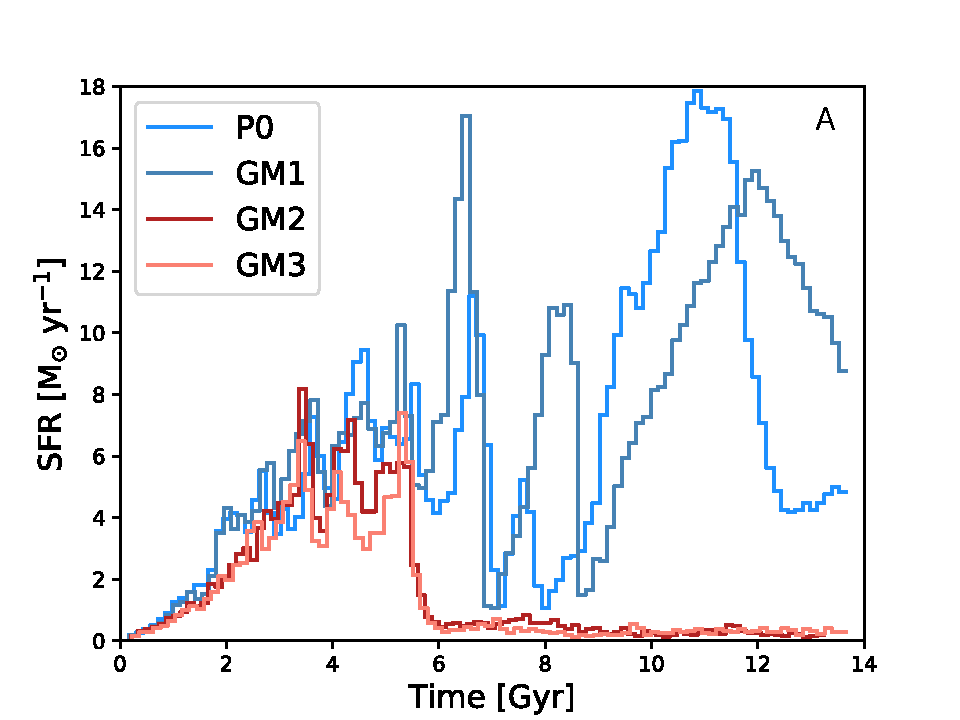
\includegraphics[angle=0]{ALLBH_sfh}}}
\vspace{-1mm}
\centerline{\resizebox{0.98\hsize}{!}{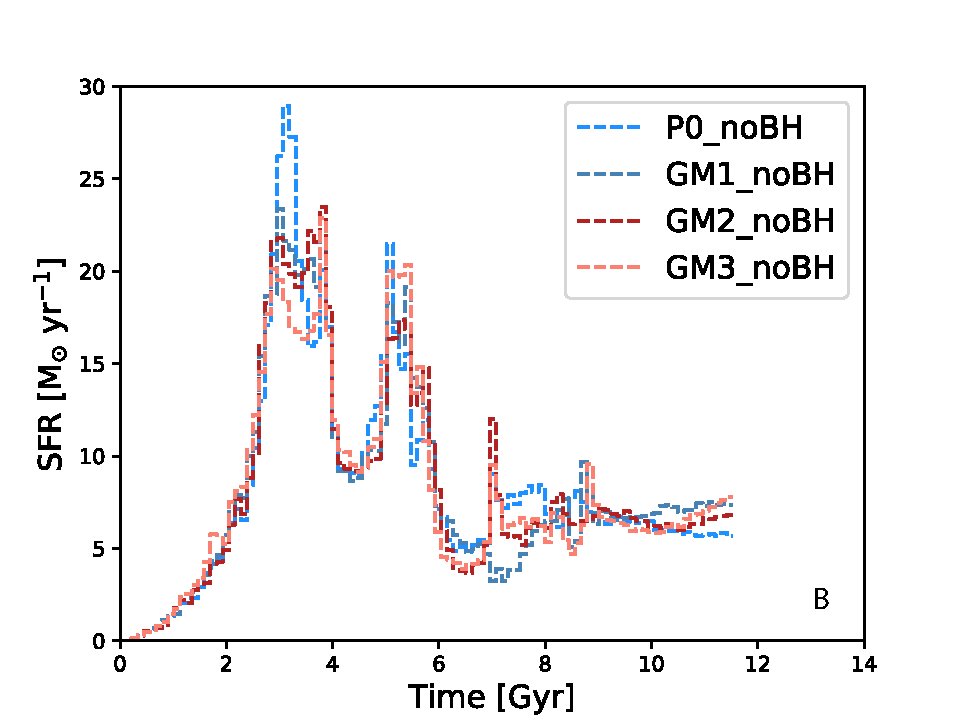
\includegraphics[angle=0]{ALLnoBH_sfh}}}
\caption[]{The star formation histories for the zoom-in galaxies: Patient 0 and its 3 GM galaxies with BH physics (\textit{Upper}) and without BH physics (\textit{Lower}). In the galaxies including BH physics, P0 and GM1 remain star forming throughout their histories while GM2 and GM3 become quenched at z $\sim$ 1. Without BH physics, all four galaxies remain star forming until z = 0.}
\label{fig-sfh}
\end{figure}

\begin{figure}[h!]
%\centerline{\resizebox{0.98\hsize}{!}{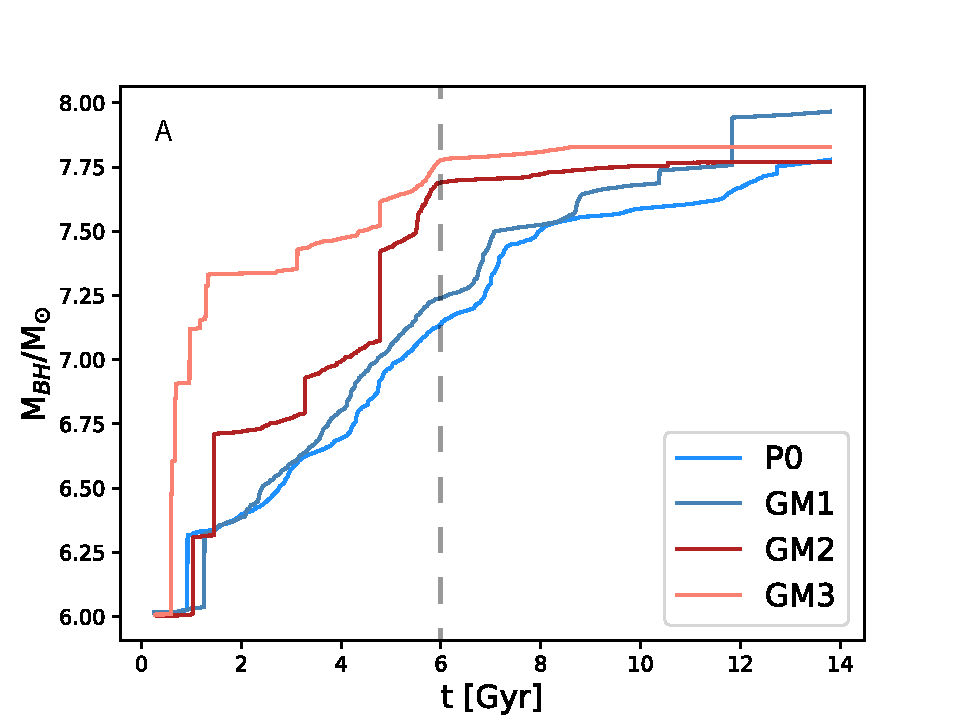
\includegraphics[angle=0]{ALLGM_BHmass}}}
%\centerline{\resizebox{0.98\hsize}{!}{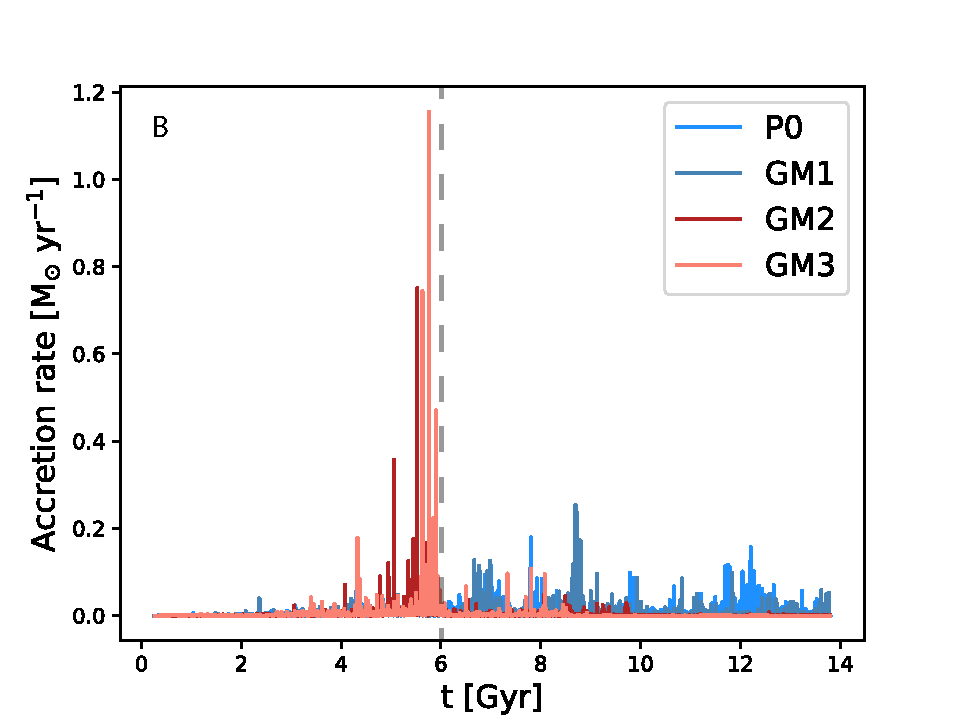
\includegraphics[angle=0]{ALLGM_BHaccrrate}}} 
\centerline{\resizebox{0.98\hsize}{!}{\includegraphics[angle=0]{ALL_bhaccrmass_age}}}
\centerline{\resizebox{1.02\hsize}{!}{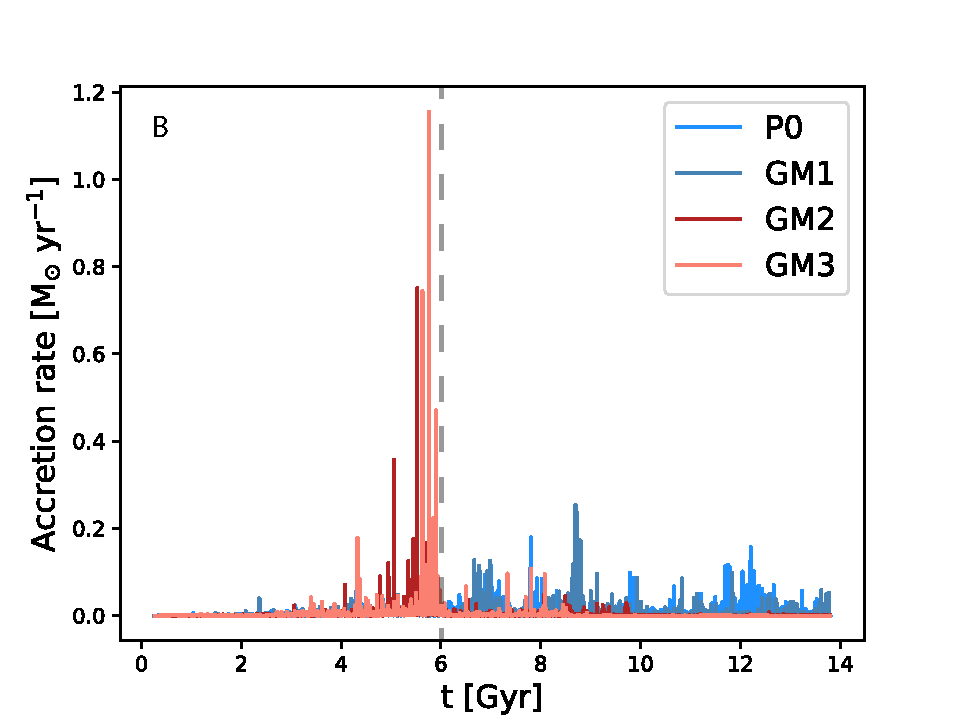
\includegraphics[angle=0]{ALLGM_BHaccrrate}}} 
\caption[]{SMBH accreted mass (\textit{Upper}) and SMBH accretion rates (\textit{Lower}) for our 4 zoom-in galaxies. Colors as in Figure \ref{fig-sfh}. The accreted mass of all the galaxies are comparable; however, both quenched galaxies also have a sharp peak in accretion rate around the time of the most significant merger (z $\sim$ 1, t $\sim$ 6 Gyr), indicated by the dashed grey line.}
\label{fig-bh}
\end{figure}

\subsubsection{Quenching in GM2 and GM3} \label{subsec-quench}
\cite{Pontzen2017a} previously explored the relationship between BH feedback and mergers and its effect on quenching, using the same genetic modification technique as we use for the GM galaxies in our study. They determine that SMBH feedback is critical to quenching a galaxy, which is consistent with our finding that the \textit{only} quenched galaxies are in simulations that include SMBHs (Figure \ref{fig-sfh}a). \cite{Pontzen2017a} argues that the merger can disrupt the cold disk of the galaxy, which then allows the feedback of the SMBH to have a farther reaching effect on the star forming gas of the disk thereby keeping the galaxy in a state of quiescence. Mergers have also been shown to help funnel gas into the region of the SMBH allowing for more direct accretion \citep{Sanchez2017}. The top panel of Figure \ref{fig-sfh} shows star formation histories of the four zoom-in galaxies with BH physics included. It demonstrates that, unlike P0 and GM1 which remain star forming throughout their history, GM2 and GM3 become quenched at z $\sim$ 1. This immediate quenching just after the merger of the satellite with the main halo \textit{does not} take place in the set of zoom-in galaxies without BH physics, as predicted by \cite{Pontzen2017a}. Contrastingly, the lower panel of Figure \ref{fig-sfh} shows the star formation histories of the four zoom-in galaxies without BH physics and all four of their histories remain star forming and are fairly similar. The stark differences between the GM2 and GM3 galaxies with and without BHs imply that some interplay between the satellite's mass and the SMBH feedback must play a pivotal role in quenching these galaxies so thoroughly. 

We further examine the effects of the BH by looking to the accreted mass and accretion rates of the BHs. The upper panel in Figure \ref{fig-bh}a shows the cumulative accreted SMBH mass as a function of time. Here we see that the accreted mass growth in the quenched galaxies, GM2 and GM3, isn't significantly different than that of the star forming galaxies. However, more significant differences arise in Figure \ref{fig-bh}b which depicts the SMBH accretion rates as a function of time. From this figure, we can see an increase of accretion occurs for both quenched galaxies near the time of the merger (z $\sim$ 1, t $\sim$ 6 Gyr). In particular, for the two quenched galaxies, we see that the accretion rate peaks about a Gyr ealier than for the star forming galaxies. Unsurprisingly, the accretion rate in the quenched galaxy continues to drop after this point, while the SMBH in the star forming galaxies continues to accrete. Though the BH's activity and growth are not directly affected by the changing mass of the incoming satellite, together the modified satellite mass and effect of the BH make a significant impact on the star formation history of the galaxy.  

We note that the genetic modifications performed on the galaxies of \citep{Pontzen2016} were different from the ones implemented here. In their case, it was an increase of the satellite's mass that resulted in a quenched galaxy, rather than a shrinking as we implement here; however, due to the lower mass satellite in our quenched galaxies, we see that the mass is compensated by faster, early accretion (Figure \ref{fig-bh}). 

This set of galaxies, which were produced from very similar initial conditions but which illustrate very different star formation and accretion histories, allows us to directly examine how assembly history may imprint itself on the CGM. Additionally, they allow us to concretely confirm the results of \cite{Pontzen2017a} that the effect of a SMBH, while not the only requisite, is \textit{vital} to the quenching process in galaxies. 

% ### END OF SIMULATION PARAMETERS ####
% #####################################


% #####################################
% ############# RESULTS ###############
% #####################################
\vspace{-3mm}
\begin{figure}[ht!]
\centerline{\resizebox{01.02\hsize}{!}{\includegraphics[angle=0]{Novi_profile_COSHalosrange_plusobs_z0_17}}}
\caption[]{Mean column densities of \ion{O}{6} as a function of radius for all 52 of the galaxies in R25 which fall within the COS-Halos stellar mass range and our family of zoom-in galaxies. All galaxies are examined at z = 0.17. Grey lines indicate R25 galaxy column densities, and black solid lines describe our four zoom-in galaxies. Filled circles and squares indicate star forming and passive galaxies from the COS-Halos Survey dataset. Unfilled markers indicate upper limits.}
\label{fig-ROM_GMs_NOvi}
\end{figure}


\vspace{-7mm}
\begin{figure}[ht!]
\centerline{\resizebox{1.\hsize}{!}{\includegraphics[angle=0]{OPPEN_fig10_ROMgxys_averaged}}}
\caption[]{Average oxygen ion fractions in the CGM of R25 within 3 M$_{halo}$ range bins: 5 $\times$ 10$^{10}$ \textemdash 5 $\times$ 10$^{11}$, 5 $\times$ 10$^{11}$ \textemdash 2 $\times$ 10$^{12}$, and 2 $\times$ 10$^{12}$ \textemdash 2 $\times$ 10$^{13}$. Log M$_{Halo}$ for each halo are labeled in white text. \ion{O}{6} is labeled in green.}
\label{fig-oppenheimer}
\end{figure}

\begin{figure}[ht!]
\centerline{\resizebox{1.1\hsize}{!}{\includegraphics[angle=0]{Novi_profile_HIGHMASSROM_plusobs}}}
\caption[]{Column density profiles of \ion{O}{6} in the high mass (M$_{vir}$ \textless 2 $\times$ 10$^{12}$ M$_{\odot}$) galaxies of R25.}
\label{fig-highmass_Novi}
\end{figure}

\begin{figure}[ht!]
\centerline{\resizebox{1.1\hsize}{!}{\includegraphics[angle=0]{ALLGMs_plusnoBH_Novi_R_grp}}}
\caption[]{Column density profiles of \ion{O}{6} in our 4 zoom-in galaxies with (solid lines) and without (dashed lines) BH physics. P0 and GM1, our two star forming galaxies are marked in light blue and dark blue, respectively. Our quenched galaxies, GM2 and GM3, are labeled in dark red and pink, respectively. These column densities show that the BH is essential to shaping the \ion{O}{6} in the CGM of star forming and passive galaxies alike.}
\label{fig-GMs_NOvi}
\end{figure}

\begin{figure*}
\centerline{\resizebox{0.45\hsize}{!}{\includegraphics[angle=0]{ALLGMs_plusnoBH_T_R_grp}}
\resizebox{0.46\hsize}{!}{\includegraphics[angle=0]{ALLGMs_plusnoBH_rho_R_grp}}}
\centerline{\resizebox{0.45\hsize}{!}{\includegraphics[angle=0]{ALLGMs_plusnoBH_Omass_R_grp}}
\resizebox{0.455\hsize}{!}{\includegraphics[angle=0]{ALLGMs_plusnoBH_Z_R_grp}}}
\caption[]{Temperature, oxygen mass, total density, and metallicity profiles of the CGM of our 4 zoom-in galaxies with and without BH physics. Colors and linestyles as in Figure \ref{fig-GMs_NOvi}.}
\label{fig-GMs_profiles}
\end{figure*}

\begin{figure}[h!]
\centerline{\resizebox{1.05\hsize}{!}{\includegraphics[angle=0]{ALLGMs_DISKmetals_R_plusnoBH_color}}}
\caption[]{Metallicity profile of the gas within the disk of our 4 zoom-in galaxies with and without BH physics. Colors and line styles as in Figure \ref{fig-GMs_NOvi}. Without the black hole physics, metals remain trapped near the center of the disk with no mechanism to propagate out into the CGM.}
\label{fig-disk_Z}
\end{figure}


\begin{figure*}[p!]
\centerline{\resizebox{0.42\hsize}{!}{\includegraphics[angle=0]{P0_phasediagram_CGMat10_CGMmass_3456_AHF}}
\resizebox{0.42\hsize}{!}{\includegraphics[angle=0]{P0noBH_phasediagram_CGMat10_CGMmass_3456_AHF}}}

\centerline{\resizebox{0.42\hsize}{!}{\includegraphics[angle=0]{GM1_phasediagram_CGMat10_CGMmass_3456_AHF}}
\resizebox{0.42\hsize}{!}{\includegraphics[angle=0]{GM1noBH_phasediagram_CGMat10_CGMmass_3456_AHF}}}

\centerline{\resizebox{0.42\hsize}{!}{\includegraphics[angle=0]{GM2_phasediagram_CGMat10_CGMmass_3456_AHF}}
\resizebox{0.42\hsize}{!}{\includegraphics[angle=0]{GM2noBH_phasediagram_CGMat10_CGMmass_3456_AHF}}}

\centerline{\resizebox{0.42\hsize}{!}{\includegraphics[angle=0]{GM3_phasediagram_CGMat10_CGMmass_3456_AHF}}
\resizebox{0.42\hsize}{!}{\includegraphics[angle=0]{GM3noBH_phasediagram_CGMat10_CGMmass_3456_AHF}}}
\caption[]{Phase diagrams of the temperature and density of the two star forming zoom-in galaxies, P0 (\textit{Top row}) and GM1 (\textit{Second row}), and the two quenched galaxies, GM2 (\textit{Third row}) and GM3 (\textit{Bottom row}). The phase diagrams of galaxies with BH hole physics vary quite widely between the star forming (P0 and GM1) and quenched cases (GM2 and GM3), particularly in the highest temperature and density gas. However, the phase diagrams of the galaxies without BH physics appear nearly identical, as are their star formation histories. Semi-transparent light and dark grey boxes span the region of collisionally and photoionized \ion{O}{6} as temperature and density regions where fractions of \ion{O}{6} are larger than 0.05 \%.}
\label{phasediagrams}
\end{figure*}

\begin{figure*}[p!]
\centerline{\resizebox{0.384\hsize}{!}{\includegraphics[angle=0]{P0_phasediagram_CGMat10_Omass_3456_AHF}}
\resizebox{0.382\hsize}{!}{\includegraphics[angle=0]{P0_phasediagram_CGMat10_metallicity_3456_AHF}}
\resizebox{0.383\hsize}{!}{\includegraphics[angle=0]{P0_phasediagram_CGMat10_Rkpc_3456_AHF}}}

\centerline{\resizebox{0.384\hsize}{!}{\includegraphics[angle=0]{GM3_phasediagram_CGMat10_Omass_3456_AHF}}
\resizebox{0.382\hsize}{!}{\includegraphics[angle=0]{GM3_phasediagram_CGMat10_metallicity_3456_AHF}}
\resizebox{0.383\hsize}{!}{\includegraphics[angle=0]{GM3_phasediagram_CGMat10_Rkpc_3456_AHF}}}

\centerline{\resizebox{0.384\hsize}{!}{\includegraphics[angle=0]{P0noBH_phasediagram_CGMat10_Omass_3456_AHF}}
\resizebox{0.382\hsize}{!}{\includegraphics[angle=0]{P0noBH_phasediagram_CGMat10_metallicity_3456_AHF}}
\resizebox{0.383\hsize}{!}{\includegraphics[angle=0]{P0noBH_phasediagram_CGMat10_Rkpc_3456_AHF}}}

\centerline{\resizebox{0.384\hsize}{!}{\includegraphics[angle=0]{GM3noBH_phasediagram_CGMat10_Omass_3456_AHF}}
\resizebox{0.382\hsize}{!}{\includegraphics[angle=0]{GM3noBH_phasediagram_CGMat10_metallicity_3456_AHF}}
\resizebox{0.383\hsize}{!}{\includegraphics[angle=0]{GM3noBH_phasediagram_CGMat10_Rkpc_3456_AHF}}}

\caption[]{Phase diagrams of the temperature and density of the star forming zoom-in galaxy, P0 and GM2 (\textit{Top two rows} with BH physics and the same two galaxies without (\textit{Lower two rows}). \textit{Left:} The phase diagrams of these galaxies weighted by the total oxygen mass in each bin. \textit{Middle:} The same phase diagram showing temperature and density, however, the colorbar is weighted by the average metallicity of the star in each bin. We note that the high density, high temperature gas we see in the star forming P0, is also the highest metallicity gas in the CGM. \textit{Right:} Similarly, a phase diagram with the colorbar now weighted by the average distance from the center of the galaxy of the gas particles in each bin.}
\label{figure:phasediagrams_z_R}
\end{figure*}

\section{Results}\label{sec-results}
% We identify halos using AHF and result in halos of this mass range.
Individual halos in the {\sc Romulus25} cosmological volume and in the individual zoom-in galaxies are extracted using the Amiga Halo Finder (AHF) \citep{Knollmann2009} and central SMBH positions and velocities are defined relative to the center position and inner 1 kpc center-of-mass velocity of their host halo, respectively. All zoom-in galaxies are isolated with their most major merger occurring at z $\sim$ 1 (mass ratio = M$_{halo}$/M$_{sat}$, q \textless 10) and their modified satellite halo still present at z = 0. An additional merger occurs (q $\sim$ 10) close to z = 0.2, though this time varies slightly across the simulations (See Section \ref{Result:metalsbyBH}).

% We define the CGM on this scale and in this environment for our galaxies.
The CGM of each individual galaxy halo (within the R25 galaxies and our zoom-ins) is defined as the mass enclosed in an annulus from 10 kpc from the center position out to a virial radius defined as the radius at which the density is 200 times the critical density, $\rho_c$, where $\rho/\rho_c$ = 200. While the genetic modification process results in galaxies with similar final masses, we find that the mass of the CGM correlates with the mass of the halo when BH physics is included. P0, which results in the most massive halo at z $\sim$ 0, has the most mass in its CGM, while GM3 results in the least massive CGM mass and halo mass (Table \ref{table:noBHdata}).


\subsection{\ion{O}{6} as a Tracer for Virial Temperature}
\label{Result:OviasTtracer}
% We calculate the column densities of \ion{O}{6} like this.
Column densities of \ion{O}{6} are calculated using the analysis software Pynbody \citep{pynbody}. Oxygen enrichment from supernovae and winds is traced throughout the integration of the simulation and ionization states are calculated during post-processing, assuming optically thin conditions, a \cite{Haardt2012} ultraviolet radiation field at z = 0, and collisional ionization equilibrium. Recent papers have raised concerns that this UV background is too weak \citep{Kollmeier2014,Shull2015}; however, as the \ion{O}{6} in our simulations is predominantly collisionally ionized, our choice of UV background does not affect our results. We use the CLOUDY software package \citep{Stinson2012,Ferland2013} to create models with varying temperature, density, and redshift to determine \ion{O}{6} fractions for all the gas in each simulated galaxy. Figure \ref{fig-ROM_GMs_NOvi}a shows the column densities of \ion{O}{6} as a function of radius for our 52 R25 MW-mass galaxies. Red and blue lines describe quenched and star forming galaxies within the sample, respectively. The COS-Halos dataset is plotted on top in black, with squares and circles distinguishing between elliptical and spiral galaxies. Upper limits are designated with arrows and unfilled markers. The R25 galaxies well match the observations from the COS-Halos Survey. We further compare the column densities of \ion{O}{6} in the R25 galaxies to the 4 zoom-in galaxies with BH physics and find that these galaxies also well match the observed column densities of COS-Halos and fall within the range of the R25 galaxies (Figure \ref{fig-ROM_GMs_NOvi}). 

Figures \ref{fig-ROM_GMs_NOvi} makes it clear that our simulations reproduce the column densities of \ion{O}{6} in the CGM. In addition, we note that \textit{the column densities of \ion{O}{6} in the CGMs of these galaxies does not depend on the assembly history of the galaxy.} We see this in both R25, which in addition to providing evidence for this initial result also gives cosmological credence to our suite of GM galaxies, and our four GM galaxies that include BH physics. We confirm our result with Patient 0 and its GMs, which include two star forming galaxies and two quenched galaxies, all of which well match the \ion{O}{6} observations despite differing assembly histories.


Figure \ref{fig-oppenheimer} shows the average ionization fractions for all the ionization states of oxygen within three mass ranges: low mass (5 $\times$ 10$^{10}$ \textemdash 5 $\times$ 10$^{11}$ M$_{\odot}$), Milky Way-mass (5 $\times$ 10$^{11}$ \textemdash 2 $\times$ 10$^{12}$ M$_{\odot}$), and high mass (2 $\times$ 10$^{12}$ \textemdash 2 $\times$ 10$^{13}$ M$_{\odot}$). The \ion{O}{6} fractions in green decrease from the MW-mass range to the high mass regime due to the increase in virial temperature which moves from a value close to the ionization peak for \ion{O}{6}, T $\sim$ 10$^{5.5} K$ to 10$^{6.3}$ K. Similarly, Figure \ref{fig-highmass_Novi} confirms that as galaxy virial mass increases, column densities of \ion{O}{6} decrease. From this study, we determine that morphological evolution of the galaxy doesn't correlate with the evolution of \ion{O}{6} in the CGM. Instead, it appears that the mass of the galaxy, as traced by its virial temperature (Table \ref{table:BHdata}), plays a more significant role in determining the column density of \ion{O}{6} seen in the CGM.

\subsection{Metal Transport by the SMBH}
\label{Result:metalsbyBH}

We examine the column densities of \ion{O}{6} in the CGMs of our 4 zoom-in galaxies \textit{without} BH physics and compare them to the cases where BH physics is included. Figure \ref{fig-GMs_NOvi} shows the column densities of \ion{O}{6} in the CGM of all four of our zoom-in galaxies with BH physics (solid lines) and without (dashed lines). We can see that in the cases where BH physics is not included, the values of N$_{OVI}$ are significantly lower implying that the presence of the SMBH must play an important role in populating \ion{O}{6} in the CGM. We look to the temperature, oxygen mass, density, and metallicity of the CGM to investigate the cause of this decrease in \ion{O}{6}. (Figure \ref{fig-GMs_profiles})

Figure \ref{fig-GMs_profiles} shows that the difference between the CGMs of these two cases appears to come directly from the change in metallicity due to the lack of black hole activity. We examine the metallicity of the disk to look for further clues about how the lack of SMBH activity is affecting the galaxy. Figure \ref{fig-disk_Z} shows that, in the galaxies without BH physics, the metals produced in the disk are not being driven into the CGM due to the lack of SMBH feedback. 

To further explore this result, Figure \ref{phasediagrams} shows the phase diagrams of the CGMs of the 4 zoom-in galaxies both with and without BH physics. Examining the CGM phase diagrams for the GMs that \text{include} BH physics (\textit{Left Column}), we note the following key differences. First, there is decreasing overall mass from the uppermost (P0) to lowermost (GM3) figure. We can attribute this difference to the slight decrease in total halo mass from P0 to GM3 (Table \ref{table:BHdata}) and to the fact that both GM2 and GM3 are quenched galaxies. 

Second, the amount of cool, dense gas (T \textless 10$^{4.5}$, n$_H$ \textgreater 10$^{-3}$) in each galaxies' CGM varies. We attribute this to various characteristics of each simulation. In particular, for P0 and GM1 with BH physics much of this gas comes from some disk gas present at our definition of the CGM boundary, R = 10 kpc. For GM7 with BH physics, this gas comes primarily from incoming satellite galaxies. We attribute the same reasoning to the 4 galaxies without BH physics which also have a similar structure in their CGM phase diagrams (as we explore further below).

Finally, there is a significant lack of hot, dense gas (T \textgreater 10$^{5.5}$, n$_H$ \textgreater 10$^{-3}$) in the phase diagrams of GM2 and GM3, our quenched galaxies. To study this final difference, we further explore the CGM phase diagrams that \textit{exclude} BH physics (\textit{Right Column}), we note that the overall shapes of these phase diagrams are similar the the star forming galaxies \textit{with} BH physics, which is unsurprising since all four of these galaxies remain star forming throughout their evolution (Figure \ref{fig-sfh}b). The similarities end there, however, as the merger histories of these galaxies are characterized by a late-z merger which occurs at slightly varying times for the 4 galaxies without BH physics. This late-z merger is separate from the modified satellite which is still present at z = 0 in each galaxy's halo.

P0 has its last significant merger (q $\sim$ 10) at z $\sim$ 0.7. GM1 has a similar minor satellite merger at z $\sim$ 0.5  which increases the amount of metal in the CGM (up to ~ 2 $\%$ compared to P0), but by z = 0.17, the satellite galaxy has merged fully with the galaxy of the main halo. Only 0.1 $\%$ of the highest metallicity gas remains outside of 20 kpc from the galaxy, or about 10$^6$ M$_{\odot}$.  In GM2, the minor satellite galaxy merger occurs at z $\sim$ 0.17 causing a large swell in the amount of metal enrichment seen in the CGM. This high metallicity gas accounts for 3 $\%$ of the total CGM gas mass and is almost entirely present, M$_{Z > 0.8 Z_{\odot}, R > 20 kpc}$ = 2.3 $\times$ 10$^{9}$ M$_{\odot}$, outside of 20 kpc from the main halo's disk (still concentrated in the region of the satellite galaxy). This satellite in GM3 doesn't fully merge with the main halo until almost z $\sim$ 0. We note that similar, late-z mergers are present in the zoom-in galaxies with BH physics; however, their effect is less significant due to the metal enrichment caused by the SMBH.

There is a lack of the hot, dense gas in the quenched galaxies that is present in the star forming galaxies, P0 and GM1. We note that this feature is also present in the CGM diagrams of the galaxies \textit{without} BH physics, which all result in star forming, disked galaxies. Figure \ref{figure:phasediagrams_z_R} further examines this difference with the same CGM phase diagrams of P0 and GM3 weighted by oxygen mass, metallicity, and distance from the center of the galaxy, with (\textit{Two Upper Rows}) and without (\textit{Two Lower Rows}) BH physics. The hot, dense gas in P0 with BH physics (\textit{Upper Row}) appears to be mostly comprised of high metallicity gas that is close to the disk (R \textless 50 kpc). Further examining this gas, we find that 3 $\%$ of the CGM gas has metallicity Z \textgreater 0.8 Z$_{\odot}$ at z = 0.17. Furthermore, of this 3 $\%$, nearly 30 $\%$ is farther than 20 kpc from the center of the galaxies. For GM1, the CGM is comprised of 6.7 $\%$ gas with Z \textgreater 0.8 Z$_{\odot}$ with 55 $\%$ of that gas farther than 20 kpc. Contrastingly, a negligible amount of the CGM of both GM2 and GM3 have Z \textgreater 0.8 Z$_{\odot}$ at z = 0.17. The CGMs of the four galaxies without BH physics also have small amounts of gas with Z \textgreater Z$_{\odot}$, from 0.2 $\%$ in P0noBH to 0.1 $\%$ in GM3noBH, when discounting the contribution from the satellite merger at z $\sim$ 0.2. These percentages of high metallicity gases in P0 and GM1 with BH physics point to metal exchange in the galaxy that is strongly dependent on the SMBH. This result is consistent with our discussion of Figure \ref{fig-disk_Z} and with \cite{Nelson2018} who also find that metal mass ejection due to the BHs in their simulations is key to their results (See Section \ref{sec-discuss} for more details).

The lack of high metallicity gas in the CGM phase diagrams of the galaxies with no BH physics (\textit{Right Column}) confirms the fact that metals are not being driven out of the disk. We find that feedback does not play a significant role in directly heating or excavating the CGM gas, but instead the SMBH's feedback is pivotal in \textit{transporting the metals} from the center of the galaxy out into the CGM. \textit{The SMBH plays a significant role in physically driving the metals out of the disk and into the outer regions of the CGM.}

%$\textbf{[Include discussion about metal flux into and out of galaxy (once complete); comparisons between observations and amount of total metals in disk (plus metal gradients)]} 


% ########## END OF RESULTS ###########
% #####################################

% #####################################
% ########### DISCUSSION ##############
% #####################################
\section{Discussion} 
\label{sec-discuss}

These results are consistent with those of \cite{Oppenheimer2016} who used a suite of EAGLE simulated galaxies to examine the bimodality of \ion{O}{6} column densities \citep[further discussed in][]{Tumlinson2011} in star forming and quenched galaxies. They argue that the star forming galaxies (M$_{halo}$ = 10$^{11}$ - 10$^{12}$ M$_{\odot}$), which were found to have a higher fraction of \ion{O}{6}, were at the right virial temperature to maximize \ion{O}{6} production, while their quenched galaxies (M$_{halo}$ = 10$^{12}$ - 10$^{13}$ M$_{\odot}$) had high enough virial temperatures such that the dominant ionization state was not \ion{O}{6} but rather \ion{O}{7} or above. \cite{Oppenheimer2016} argues that the \ion{O}{6} content was not a tracer of star formation directly, but rather a more direct thermometer for the temperature of the halo.

We note that the quenched galaxies in our sample have slightly smaller halo masses than our star forming galaxies, unlike those in Oppenheimer, explaining the lack of bimodality that we observe. While all 4 of our zoom-in galaxies (with BH physics) are in the mass range to have virial temperatures which optimize \ion{O}{6}, we further examine the R25 simulation's higher mass, passive galaxies in addition to the MW-mass galaxies (which have virial temperatures spanning 5.8 $\times$ 10$^{5}$ K \textemdash 1.1 $\times$ 10$^{6}$ K) to see if the bimodality appears. Figure \ref{fig-highmass_Novi} directly shows that the column densities of \ion{O}{6} still act as thermometer for the temperature of the halo as argued by \cite{Oppenheimer2016}.

Furthermore, examining galaxies within low, MW-, and high mass bins from the R25 suite, we see that the column densities of \ion{O}{6} decrease as the ionization peak of \ion{O}{6} is surpassed by these halos. Since the virial temperature is higher, the oxygen is likely to be ionized to a higher ionizations state (\ion{O}{7} or \ion{O}{8}), which we show is the case in Figure \ref{fig-oppenheimer}. 

This lack of bimodality run contrary to the findings of \cite{Suresh2017} and \cite{Nelson2018}, both of which attribute such an affect to the SMBH feedback in their simulations. We see no such affect, particularly in our 4 zoom-in galaxies which act as a test case for different accretion histories moderated by the effect of a shrunken satellite mass. The resulting zoom-ins all have very similar characteristics (Table \ref{table:BHdata} and Figure \ref{fig-bh}) and we do not see much difference between their column densities of \ion{O}{6}. We do, however, find consistency with \cite{Nelson2018} which argues that the SMBH is responsible for enriching the CGM by physically driving metals out of the disk, as we see in our simulations. 

With this study, we add to the growing reservoir of data suggesting that the evolution of the CGM and SMBH are tied together. While many studies both theoretical and observational have been interested in connecting the star formation and galactic accretion history to CGM properties, there has been no observational study that has yet tied CGM measurements to SMBH properties. Future observations of the CGM in galaxies with well-known SMBH masses could attempt to solve this mystery. Figure \ref{fig-BHmass} shows our prediction for baryon fractions in the inner CGM of our 52 R25 galaxies within the COS-Halos stellar mass range. We find a significant trend between a decrease in baryon fraction in the inner CGM as the mass of the central SMBH increases. Therefore, we predict that galaxies with larger SMBH will have more evacuated CGMs.



% ########## END OF DISCUSSION ###########
% ########################################


% #####################################
% ########### CONCLUSION ##############
% #####################################

\begin{figure}[ht!]
\vspace{-3mm}
\centerline{\resizebox{1.1\hsize}{!}{\includegraphics[angle=0]{Mgasoverbaryons_BHmass}}}
\caption[]{Baryon fraction in the inner CGM (10 \textemdash 100 kpc) for the 52 R25 galaxies within the COS-Halos stellar mass range as a function of SMBH mass. Points are weighted by stellar mass of each galaxy.}
\label{fig-BHmass}
\end{figure}

\section{Conclusion}
\label{sec-conclude}

Using the cosmological volume {\sc Romulus25} and a zoom-in galaxy with 3 genetic modification run with and without BH physics, we have examined the effects of SMBH feedback and star formation history on the column densities of \ion{O}{6} in the CGM of galaxies with stellar masses between 3 $\times$ 10$^{10}$ \textemdash 3 $\times$ 10$^{11}$ M$_{\odot}$.

We determine that the SMBH acts a physical driver for metal mass in the CGM. Previous studies have examined the effect of heating on the CGM as the SMBH's energy input may put the gas into phases which optimize the production of \ion{O}{6} \citep{Suresh2017}.  Others have proposed that the feedback from SMBH may physically drive outflows of gas out of the galaxy, resulting in a lower density CGM and therefore lower densities of \ion{O}{6} \citep{McQuinn2017,Mathews2017}. However, neither of these cases are what we see. \textit{Instead, we see a set of galaxies with CGMs which rely on the SMBH for the propagation of metal mass (but not total gas mass) into the outer galaxy and \ion{O}{6} columns which depend on the virial temperature of the galaxy} (Figure \ref{fig-disk_Z}). This result is consistent with those of \cite{Oppenheimer2016} and \cite{Nelson2018}; however, the latter argue that the bimodality of N$_{OVI}$ between star forming galaxy and quenched galaxy is a result of SMBH feedback, which we do not see.

The combined, consistent results of the cosmological R25 and our zoom-in galaxies with BH physics imply a mechanism by which column densities of \ion{O}{6} are set by the virial temperature of the CGMs host galaxy, and are not significantly affected by the evolution of a disk. Their phase diagrams also show significant difference in response to their overall assembly history, showing more, higher metallicity gas in the star forming cases. Nevertheless, the column densities of \ion{O}{6} remain consistent despite differences in star formation history and the significant variations of their phase diagrams. Therefore, we surmise that the differences in the CGM are not determined by whether or not a galaxy quenches but rather the conditions for \ion{O}{6} are primarily set by the amount of metals propagated into the disk by the BH and the virial temperature of the galaxy.


% ####### END OF CONCLUSIONS ##########
% #####################################

\acknowledgments
Acknowledgements

\bibliography{/Users/noodle/Documents/MENDELEY/MEND_bibtexfiles/SanchezCGM2018.bib}
% ADD THIS LATER TO BIB
% @misc{pynbody,
%   author = {{Pontzen}, A. and {Ro{\v s}kar}, R. and {Stinson}, G.~S. and {Woods},
%      R. and {Reed}, D.~M. and {Coles}, J. and {Quinn}, T.~R.},
%   title = "{pynbody: Astrophysics Simulation Analysis for Python}",
%   note = {Astrophysics Source Code Library, ascl:1305.002},
%   year = 2013
% }

\end{document}
